{A fuel oil storage tank is 10 ft deep with trapezoidal sides, 5 ft at the top and 2 ft at the bottom, and is 15 ft wide (see diagram below). Given that fuel oil weighs 55.46 lb/ft$^3$, find the work performed in pumping all the oil from the tank to a point 3 ft above the top of the tank.

\hfill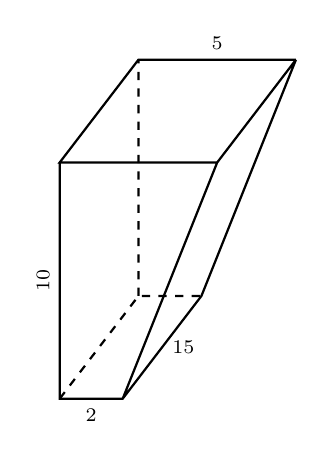
\begin{tikzpicture}[x={(1,0)},z={(0,1)},y={(.5,.87)},xscale=.4,yscale=.3]
\draw [thick] (0,0,0) -- node [above,rotate=90,pos=.5] {\scriptsize 10} (0,0,-10) --  node [below, pos=.5] {\scriptsize 2} (2,0,-10) -- node [right, pos=.5] {\scriptsize 15} (2,5,-10) -- (5,5,0)
							(5,5,0) -- (5,0,0)
							(5,0,0) -- (0,0,0) -- (0,5,0) --  node [above,pos=.5] {\scriptsize 5}(5,5,0)
							(5,0,0) -- (2,0,-10);						

\draw [thick,dashed] (0,0,-10) -- (0,5,-10) -- (2,5,-10)
																	(0,5,-10) -- (0,5,0);
\end{tikzpicture}\hfill\null
}
{212,135 ft--lb
}
